\chapter{Experiments}
\section{Environments}
Before diving into the experiments, the symmetric environments are outlined below.
\section{CartPole}\label{sec:cartpole}
\begin{figure}[h!]
	\centering
	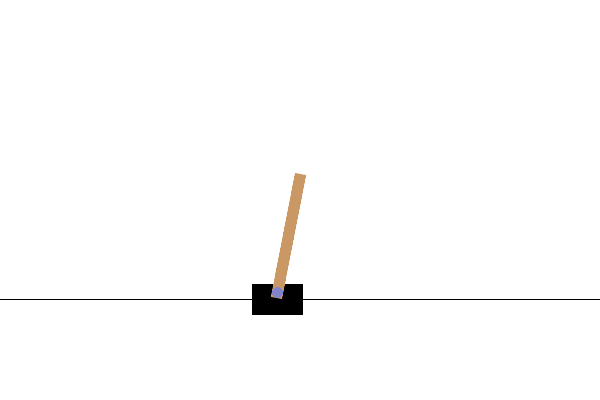
\includegraphics[width=0.5\textwidth]{Figures/cart_pole.png}
	\caption{The CartPole environment.}
\end{figure}
The CartPole environment is the "Hello World" of reinforcement learning; it describes a game where at each timestep, the aim is to balance a mass above a slider, 1 point is given for each timestep that the mass makes an angle of fewer than 12 degrees from vertical, in this instantiation. The action space$a \in {0,1}$ indicates pushing the pole left or right. The state space is the position of the cart, the velocity of the cart, the angle of the pole and the angular velocity of the pole. A state is a vector s:
\begin{equation}
	s = \begin{pmatrix}
		x       \\
		\dot{x} \\
		\theta  \\
		\dot{\theta}
	\end{pmatrix}
\end{equation}
Thus, $s \in \mathbb{R}^4$.

Typically, the episodes are truncated at 500 timesteps, and the reward is 1, so the return is an integer $G_0 \in [0, 500]$. An episode terminates if the pole falls over or the cart moves too far from the centre. If a human were learning to solve this problem, one would notice that the expected result of pushing the cart left when it is leaning right at some positions is the same as pushing the cart right when it is leaning left at the displacement in the opposite direction. This is an example of symmetry in the problem, and it is this symmetry that is exploited by~\cite{vanderpol2020mdp, mondal2020group}.

To learn the transition dynamics of CartPole and agent must learn how the system evolves through time. In CartPole the transitions between different states in CartPole are governed by the PDEs:

\begin{equation}
	\ddot{\theta} = \frac{g \sin \theta + \cos\theta \left({\frac{-F - m_p l \dot{\theta}^2 \sin(\theta)}{m_c + m_p}} \right )}{l\left ( \frac{4}{3} - \frac{m_p \cos^2 \theta}{m_c + m_p}\right)},
\end{equation}

\begin{equation}
	\ddot{x} = \frac{ F + m_p l (\dot{\theta}^2 \sin \theta - \ddot{\theta} \cos \theta)}{m_c + m_p}.
\end{equation}
Here $g$ is the acceleration due to gravity and is positive, $\theta$ is the angle between the pole and vertical, with the pole length $l$. $F$ is the action force, where the positive direction is right. The masses of the cart and the pole are $m_c, m_p$, respectively. Finally, $\dot{}$, indicates a derivative with respect to time.

These PDEs have no closed solution and their form is taken from \cite{florian2007correct} who provides slight corrections to the original dynamics in \cite{barto1983neuronlike}.

Both learning a policy and a transition model may be augmented by exploiting symmetry. The symmetry present in CartPole is the cyclic $C_2$ group. Other than the trivial group, the group with a single element, the $C_2$ group, is the simplest. This is a group with only two elements, the identity and inversion.
\begin{table}[h!]\label{tab:c2}
	\centering
	\begin{tabular}{c | c  c}
		$C_2$ & $e$ & $r$ \\
		\hline
		$e$   & $e$ & $r$ \\
		$r$   & $r$ & $e$
	\end{tabular}
	\caption{The $C_2$ group table, where entry $i, j$ is the result of group operation on the $i^{th}$ and $j^{th}$ element.}

\end{table}


%%As such, to find the group structured MDP homomorphism, the agent needs to learn an equivariant mapping that respects $\pi_1^s\mathbf{s} = \mathbf{s}$ and $\pi_r^s\mathbf{s} = -\mathbf{s}$, as well as $\pi_1^a\mathbf{a} = \mathbf{a}$ and $\pi_r^a\mathbf{a} = 1 - \mathbf{a}$. Here the state and actions as vectors; $\mathbf{s}, \mathbf{a}$ are being acted upon by the vector representations of $C_2, \pi$ in their respective spaces.

\section{Catch}\label{sec:catch}
\begin{figure}[h!]
	\label{fig:catch_env}
	\centering
	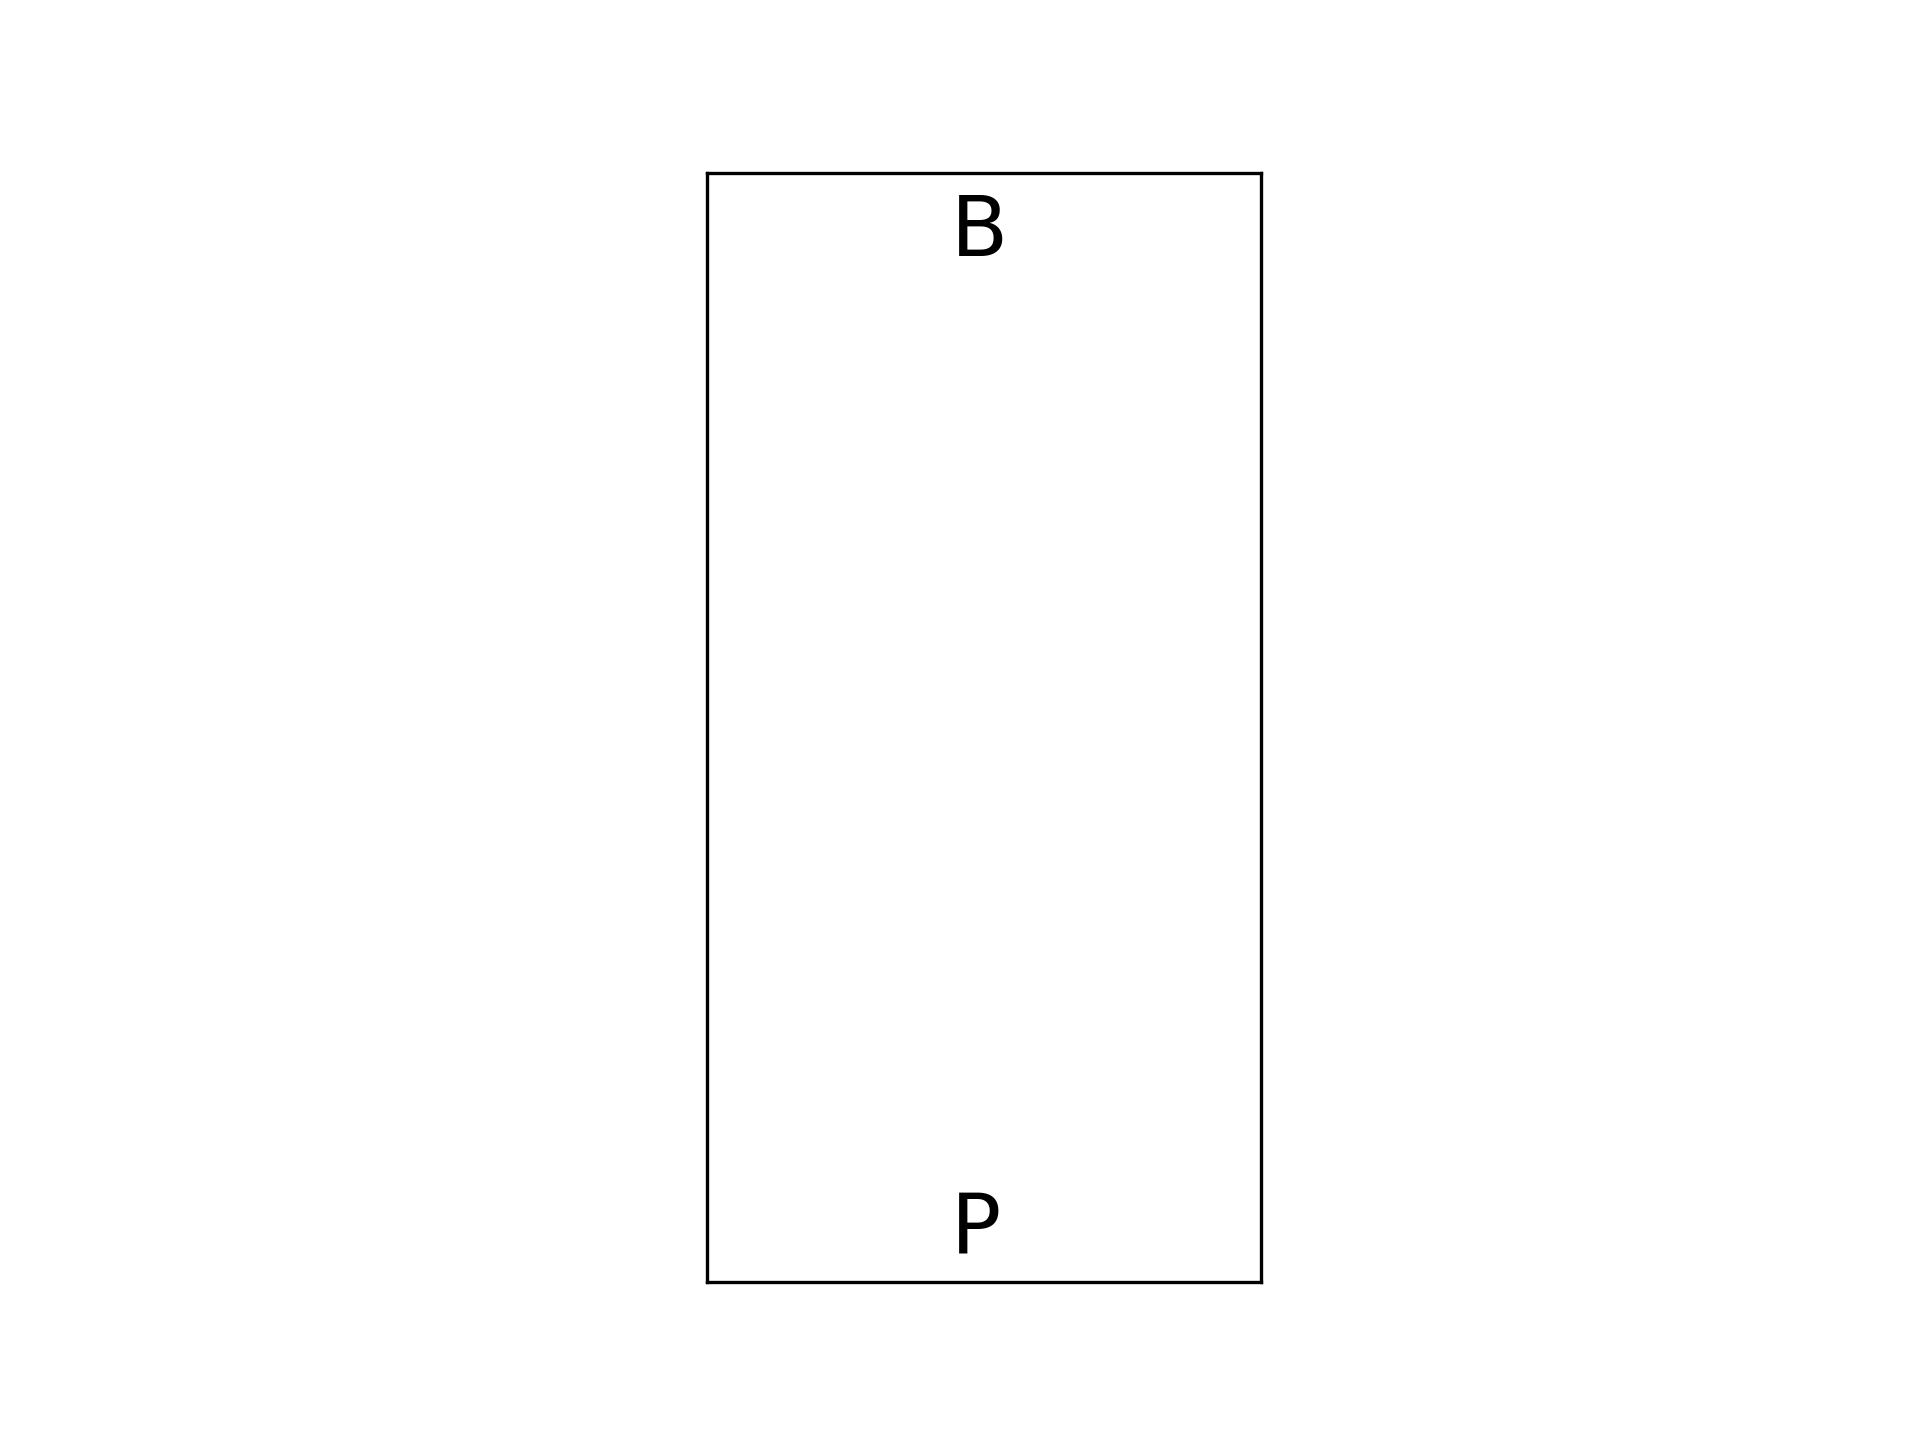
\includegraphics[width = 0.6\textwidth]{Figures/catch_env.png}
	\caption{The Catch environment. The ball position is indicated by B, and the paddle position is indicated by P.}
\end{figure}
The Catch environment~\cite{osband2020bsuite} is another simple MDP task similar to CartPole used mainly for debugging implementations. The aim of the game is to catch a falling ball. The default implementation has ten rows and 5 columns. The ball moves down by one row every time-step, and the position of the paddle is translated left or right by the action of the agent. When the ball reaches the tenth row, the reward of the system is $+1$, if the ball and the paddle are in the same location, otherwise the reward is $-1$. For all other time-steps the reward is 0. This produces an episodic environment, with a maximum return of $1$.

The state and action spaces are both discrete, and the transitions are deterministic. These states are represented to the agent as a $5\times 10$ array, with the ball and paddle's positions indicated by ones. The actions the agent can take are $\mathcal{A} = [0, 1, 2]$, that translate the ball by $1-a$. Thus, the MDP has a finite amount of transitions and state action pairs, 675 in total.

Like CartPole, the Catch environment possesses $C_2$ group symmetry, however, due to the different state and action spaces the representations of the groups are different. However, because the groups are the same the structure is that in Table.\ref{tab:c2}.

\section{Motivation}
A series of Experiments were carried out to investigate the efficacy of equivariant transition model structure in model-based RL problems with symmetric environments. Where the specific model-based algorithm investigated was Dyna.

Model-based RL, is inherently more complex than actor-critic or value based methods, as not only does a policy need to be learned, but also a model of the environment dynamics must also be learned. In the case of a NN model, this will require training a model, as well as an agent.

Even with the simple models constructed here, the model based agents have two times more parameters. Within wider literature, models such as Dreamer-v3~\cite{hafner2023mastering}, use 8 million parameters, and multiple GPU days to learn policies on the complete Bsuite~\cite{osband2020bsuite} environment.

The increased complexity in the Dyna algorithm is mitigated by its modularity. The Dyna agent is constructed out of a transition model and a model-free agent. This provides a sensible progression for development and experimentation. Firstly, the model-free agent was constructed, and the symmetric inductive biase was tested only for the agent. Then, transition models were trained offline and tested. Finally these disjoint pieces were brought together to form the full Dyna implementation.

\section{Baseline}\label{sec:baseline}
The baseline that was chosen was a proximal policy optimization, Sec.\ref{sec:PPO}, agent from PureJaxRL,~\cite{lu2022discovered, schulman2015highdimensional}. This baseline provides a training framework, that trains a single agent concurrently on multiple identical environments. The training regime is outlined below in pseudocode.
\begin{algorithm}
	\caption{PureJaxRL PPO Agent Training Structure}
	\begin{algorithmic}
		\State Initialize agent: actor-critic $\pi_\theta$, $v_\phi$
		\State Initialize replay buffer: $\mathcal{D}$
		\For{Num Updates}
		\State Gain experience for Num Timestep
		\State Store trajectories: $\mathcal{D}$.append($(S, A, S', R))$
		\State Calculate GAE estimate from experience timesteps
		\For{ Num Epochs}
		\State{ Split GAE estimates into minibatches}
		\State{ Mini-Batch SGD with Adam on $\pi_\theta, v_\phi$}
		\Comment{ See~\ref{sec:PPO} for losses to optimize}
		\EndFor
		\EndFor
		\State Returns($\mathcal{D}$)

	\end{algorithmic}
\end{algorithm}

\section{Equivariant Actor-Critics}\label{sec:actor-critic}
\subsection{CartPole}

To form an equivariant network to the group structure of CartPole the actor network must be equivariant to both the identity and inversion operator. This report provides structures for equivariant G-CNNs for both CartPole and Catch, that can easily be extended to other environments with known discrete symmetries.

\subsubsection{Constructing a CartPole Actor-Critic}
In this section, the outline for the network design is described. In the Catch section, Sec.\ref{sec:catch_ac}, a more detailed description of how to extend the procedure to other groups is outlined.
The group for CartPole contains two unique elements, in both state and action space. In state space the inversion and identity operator $e, r$ are,
\begin{equation}
	\ell^\mathcal{S}_e =
	\begin{pmatrix}
		1 & 0 & 0 & 0 \\
		0 & 1 & 0 & 0 \\
		0 & 0 & 1 & 0 \\
		0 & 0 & 0 & 1 \\
	\end{pmatrix},
	\ell^\mathcal{S}_r =
	\begin{pmatrix}
		-1 & 0  & 0  & 0  \\
		0  & -1 & 0  & 0  \\
		0  & 0  & -1 & 0  \\
		0  & 0  & 0  & -1 \\
	\end{pmatrix}.
\end{equation}
Then the action space, the inversion and identity operator are,
\begin{equation}
	\ell^\mathcal{A}_e =
	\begin{pmatrix}
		1 & 0 \\
		0 & 1 \\
	\end{pmatrix},
	\ell^\mathcal{A}_r =
	\begin{pmatrix}
		0 & 1 \\
		1 & 0 \\
	\end{pmatrix}.
\end{equation}
Thus, to parametrize an equivariant actor network, the network $\pi_\theta$ must satisfy,
\begin{equation}
	\pi_\theta(\ell^\mathcal{S}_e s) = \ell^\mathcal{A}_e \pi_\theta(s),
\end{equation}
\begin{equation}
	\pi_\theta(\ell^\mathcal{S}_r s) = \ell^\mathcal{A}_r \pi_\theta(s).
\end{equation}
Instead of using a G-CNN for the Actor-Critic, a simpler solution involves employing a network with only odd operations, such as the tanh activation, and excluding biases for all hidden representations. By definition, odd functions are equivariant to both inversion and identity transformations, ensuring the network's equivariance. However, this doesn't address the issue of equivariance in the action space. To bridge this gap, a group convolution layer is incorporated to map between representations.

The network can be considered as a composition of $f_\theta : \mathcal{S} \rightarrow \mathbb{R}^{|H|}$, an odd embedding MLP and $gc_\theta: \mathbb{R}^{|H|} \rightarrow \mathbb{R}^{\mathcal{A}}$ a group convolution layer that ``lifts" the equivariance to the action space. As such the parametric policy is,
\begin{equation}
	\pi_\theta(s) = gc_\theta(f_\theta(s)).
\end{equation}
The equivariance properties of the sub-networks with respect to the inversion operator are,
\begin{equation}
	f_\theta(-s) = -f_\theta(s),
\end{equation}
\begin{equation}
	gc_\theta(-x) =
	\begin{pmatrix}
		0 & 1 \\
		1 & 0 \\
	\end{pmatrix}
	gc_\theta(x),
\end{equation}
Where $gc_\theta(x) = [P(A=a_0), P(A=a_1)]$ describes the distribution over the binary actions of CartPole.

This G-CNN network for policy learning is the first novel contribution of this report. In comparison to the work of \cite{mondal2020group}, the policy learning G-CNN is fully equivariant, rather than learning action values from an equivariant embedding. Additionally, the network parametrizes a policy directly rather than Q values. Due to the network's end to end equivariance in comparison to the Q-value network proposed by \cite{mondal2020group}, agents parametrized by this network must take the same actions in states that are in the same orbit, which is not the case for the Q-value network, which only has an equivariant embedding. Thus, they do not guarantee equivariance in the policy.

Further, this network architecture has advantages over Symmetrizer networks, \cite{vanderpol2020mdp}, in that it does not require a large matrix inversions to solve for the parameters of the network, while still maintaining the same equivariance qualities.

\subsubsection{Results: Training Dynamics On the CartPole Benchmark}
With the network's structure established, the benchmark task focuses on mastering an expert policy within the CartPole environment. By default, CartPole imposes a maximum episode length of 500 interactions. All non-terminal states yield a reward of +1, setting the maximum episodic return at 500. As with most traditional RL problems, the primary objective in CartPole is to optimize the agent's episodic return. Finding an expert policy in CartPole using standard deep learning methods is relatively straightforward and primarily serves as an implementation benchmark. For an equivariant network structure to truly enhance the quality of the learned policy, it should strive to approach the 500 episodic return benchmark with fewer environment interactions.

When comparing the learning dynamics of policy agents, it's crucial to ensure not just that the agent achieves expertise in the task but also that the policy learning procedure remains stable across multiple random seeds. A random seed refers to the initial state in which both the agent and environment begin. Keeping training stability in mind, examining the performance under the least favourable random seeds is informative about the training robustness. If an algorithm is particularly sensitive to its initialization, its performance may be significantly impacted, and may not converge over multiple random seeds~\cite{henderson2018deep}.

For all experiments, we utilize a standard MLP for the critic without imposing any equivariance constraints. While this setup might not yield optimal performance, it's essential to highlight that training is conducted across 128 random seeds to ensure the stability of the agent's learning.

Due to constraints on the equivariant network structures, it's not always feasible to maintain an identical number of parameters across networks. In instances where the exact parameter count differs, we ensure that the depth of all networks remains constant. We then adjust the width to achieve a parameter count that's within 10\% of the MLP baseline.

Refer to Fig.\ref{fig:cp_equi_ac} below, where the mean episodic return of three agents with distinct network architectures is illustrated. Despite the differences in their structures, all networks share the same training hyperparameters, as provided in the PureJaxRL\cite{lu2022discovered} baselines. The three networks depicted are the MLP baseline from PureJaxRL, an implementation of the Symmetrizer network from \cite{vanderpol2020mdp}, and the G-CNN policy network introduced in this report.

\begin{figure}[H]
	\centering
	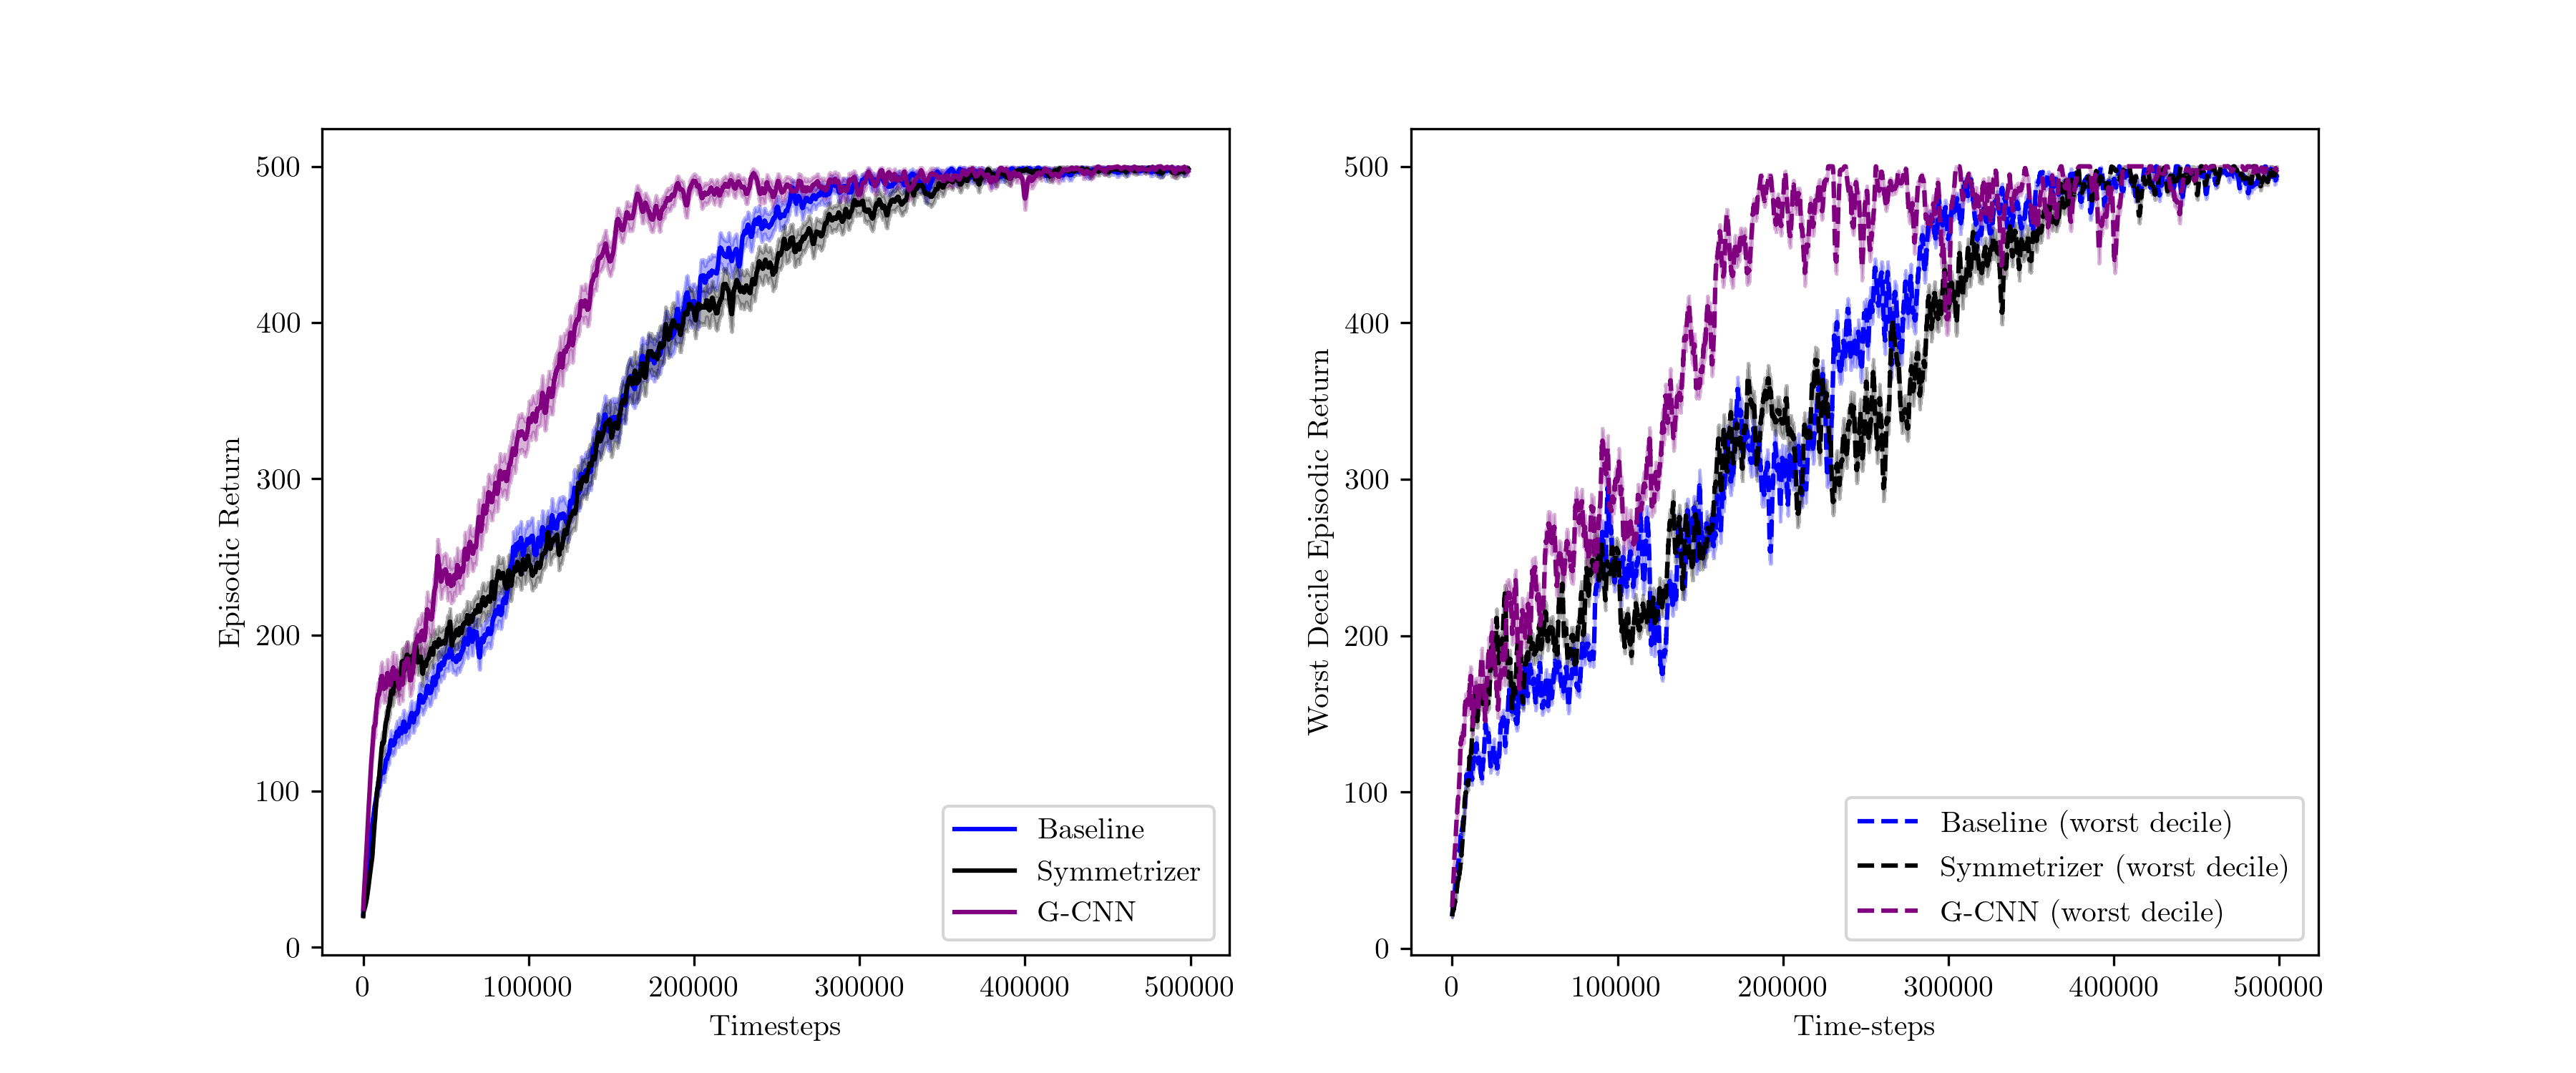
\includegraphics[width=\linewidth]{Figures/cart_pole_returns.png}
	\caption{Left: Mean episodic returns for the CartPole agents across 128 random seeds plotted against number of experience time-steps in the MDP. Right: The mean cumulative episodic returns of the worst performing 128 random seeds against number of experience time-steps in the MDP. Both of the plots are moving averages, with windows of 10 time-steps. Additionally, all plots have two standard errors plotted. } \label{fig:cp_equi_ac}
\end{figure}

Both the Symmetrizer and the G-CNN are equivariant to the actions of the $C_2$ group. This equivariance constraint requires a learned policy that respects the inversion symmetry present in Cart-pole. The equivariance  should improve the sample efficiency of the agent as any learning from one state additionally informs the agent about the agent about the policy for the other state in the orbit. This hypothesis, is supported somewhat by the observed training dynamics. Over the first period of training, both the Symmetrizer and the G-CNN, outperform the baseline. The Symmetrizer, does not maintain this performance advantage. Our implementation uses the same network size, as the original paper and the same network hyperparameters. Despite this, the Symmetrizer agent fails to learn an expert policy in fewer steps than that of the baseline.

It should be noted that here the mean plus minus two standard deviations is plotted in comparison to the median and upper and lower quartiles of cumulative returns, which is plotted in \cite{vanderpol2020mdp}. The performance of the Symmetrizer, is underwhelming despite the implemented network being checked for equivariance. Further tuning of the hyperparameters may yield performance that improves upon the baseline's returns. However, this was not a primary concern in this report.

The G-CNN does compare favourably with the baseline implementation of an MLP, having slightly fewer parameters. It can be seen that it both converges on average to an expert policy in fewer time-steps but also has a more favourable convergence behaviour in challenging initialization conditions. This can be seen in the right of Figure \ref{fig:cp_equi_ac} where, the bottom tenth percentile of cumulative returns, still converges notably faster than that of the baseline.

\begin{table}
	\centering
	\begin{tabular}{|c|c|c|c|}
		\hline
		Time-steps & Baseline     & Symmetrizer          & G-CNN                 \\
		\hline
		$10, 000$  & $102 \pm 5$  & $116 \pm 6$          & $\mathbf{158 \pm 8}$  \\
		$100, 000$ & $260 \pm 10$ & $240 \pm$ 10         & $\mathbf{330 \pm 10}$ \\
		$500,000$  & $497 \pm 1$  & $\mathbf{500 \pm 1}$ & $499 \pm 1$           \\
		\hline
	\end{tabular}
	\caption{Cumulative episodic returns tabulated for the three network architectures. All episodic returns are recorded with confidence intervals of two standard errors across 128 random seeds.}
	\label{tab:actor-critic}
\end{table}
Additionally, the mean episodic returns across all random seeds are tabulated at $10,000$, $100,000$, and $500,000$ time-steps in Table \ref{tab:actor-critic}. Upon closer inspection, the G-CNN agent incorporating the equivariant inductive bias significantly outperforms the baseline.

While both models have similar parameter counts, the structure of the G-CNNs makes their forward passes more computationally intensive. This is due to the G-CNN architecture requiring twice as many operations in a forward pass, attributed to the two group actions. However, in a scenario like Cart-Pole, where the networks are relatively small and inexpensive to evaluate—and where computation can be efficiently parallelized—both models can train 128 random seeds in under a minute. This speed is achieved using the hyperparameters listed in the Appendix and executed on a RTX 3090.

Encouraged by the promising results from the initial experiment, we decided to explore a new environment to determine whether the equivariance constraint could further enhance performance.

\subsection{Catch}\label{sec:catch_ac}
To demonstrate that G-CNN actor-critic can be extended to other environments with different group actions, we implemented the equivariant actor-critic for the Bsuite Catch environment~\cite{osband2020bsuite}. For the Catch environment, constructing an equivariant network is challenging.

\subsubsection{Constructing a Catch Actor-Critic}
Unlike the CartPole case where layers can be made equivariant to the
representation, in Catch, the entire network must be built using Group Convolutions. As in previous scenarios, we impose an equivariant constraint on the actor $\pi_\theta(s)$.
In the context of Catch, the input state space is represented as $\mathcal{S} \in [0, 1]^{50}$. Instead of detailing the cumbersome $\ell_r^\mathcal{S} \in \mathcal{R}^{50 \times 50}$ matrix representation of the reflection group action $\ell_r^\mathcal{S}$, it is left symbolically. This action modifies the x-coordinate of both the ball and the paddle using the transformation $r(x)=-(2-x)$. Thus, the equivariance constraint is expressed as:
\begin{equation}
	\pi_\theta(\ell_r^\mathcal{S} s) = \begin{pmatrix}
		0 & 0 & 1 \\
		0 & 1 & 0 \\
		1 & 0 & 0 \\
	\end{pmatrix}\pi_\theta(s).
\end{equation}
% To demonstrate that G-CNN actor-critics extend to other environments, with different group actions. The equivariant actor-critic is implemented for the Bsuite~\cite{osband2020bsuite} Catch environment. In the case of the Catch environment to make an equivariant network because layers themselves are not easily made equivariant to the C2 representation, like in the case of CartPole, the whole network must be constructed out of Group Convolutions. As before, we consider equivariant constraint on the actor $\pi_\theta(s)$.
%
% In the case of catch the input state space is $\mathcal{S} \in [0, 1]^{50}$. Avoiding writing out the tedious matrix representation of the reflection action $r$, it is left as $\ell_r^\mathcal{S}$. This action takes the x co-ordinate of the ball and the paddle and transforms them by, $r(x) = -(2-x)$. Thus, the equivariance constraint is,
% \begin{equation}
% 	\pi_\theta(\ell_r^\mathcal{S} s) = \begin{pmatrix}
% 		0 & 0 & 1 \\
% 		0 & 1 & 0 \\
% 		1 & 0 & 0
% 	\end{pmatrix}\pi_\theta(s).
% \end{equation}

To construct a G-CNN, which is equivariant to the group actions a group action in the hidden layers must be determined. Consider a group convolution input layer $f : \mathcal{S} \rightarrow \mathcal{H} \in \mathbb{R}^{|G| \times |H|}$, commonly referred to as a lifting layer that maps from a state space to a hidden space of $H$. Lifting layers apply a group action to the input and then passes the transformed input through, $ g: \mathcal{S} \rightarrow \mathbb{R}^{|H|}$, a dense/convolution layer. In the full layer the input is transformed by every group action, and then passed through $g$. In the absence of any pooling, this gives a hidden representation, that is the hidden dimensions of the equivalent dense/convolution layer, plus a new axis that is the size of the group. To illustrate the new equivariance constraint a single layer;
\begin{equation}
	g(s) = \vec{h} \in \mathbb{R}^{|H|}.
\end{equation}
When formed into a group convolution,
\begin{equation}
	f(s) = \begin{pmatrix}
		g(s)                   \\
		g(\ell_1^\mathcal{S}s) \\
		g(\ell^\mathcal{S}_2s) \\
		\vdots                 \\
		g(\ell_{|G|}s).
	\end{pmatrix}
\end{equation}
Once a group action is applied to the input, the output values undergo permutation. While the exact permutation is contingent on the group, the permutations' structure can be readily determined due to group closure:
% When a group action is applied to the input the values of the output are permuted. The exact permutation depends upon the group, however, the structure of the permutations are easily calculated due to group closure;
\begin{equation}\label{eq:gs_perm}
	f(\ell_n^\mathcal{S}s) = \begin{pmatrix}
		g(\ell_n^\mathcal{S}s)                   \\
		g(\ell_n^\mathcal{S}\ell_1^\mathcal{S}s) \\
		g(\ell_n^\mathcal{S}\ell_{|G|}s)         \\
		\vdots                                   \\
		g(\ell_n^\mathcal{S}\ell_{|G|}s)         \\
	\end{pmatrix}
	= \begin{pmatrix}
		g(\ell_n^\mathcal{S}s) \\
		g(\ell_i^\mathcal{S}s) \\
		g(\ell^\mathcal{S}_js) \\
		\vdots                 \\
		g(\ell_{k}s).
	\end{pmatrix}
	= \mat{P}_n f(s)
\end{equation}
Where $\mat{P}_n$, is a permutation matrix defined by the group. There is a unique permutation matrix for each group element. This permutation relation enables one to construct further equivariant layers. Consider a subsequent, $h: \mathcal{H} \rightarrow \mathcal{H}'$, a hidden layer that must continue the equivariance to group G. This is achieved by treating each $\mat{P}$ as the group action, and ensuring that the output is equivariant to its application. The new layer can be through of as taking a vector of responses, where it must be equivariant to the vectors' permutation,
\begin{equation}
	h\left( \mat{P_i}
	\begin{pmatrix}
		v_1    \\
		v_2    \\
		\vdots \\
		v_{|G|}
	\end{pmatrix}
	\right) = \mat{P_i} h
	\begin{pmatrix}
		v_1    \\
		v_2    \\
		\vdots \\
		v_{|G|}
	\end{pmatrix}.
\end{equation}
Tying this to a concrete example in a 1D convolution, if there is an input that is one hot, and the kernel has a single weight, $w_1$. The output of the layer will be;
\begin{equation}
	\text{Conv1D}\begin{pmatrix}
		0 \\
		1 \\
		0 \\
	\end{pmatrix}
	= \begin{pmatrix}
		0   \\
		w_1 \\
		0   \\
	\end{pmatrix}
\end{equation}
If the input is translated the output is also translated;
\begin{equation}
	\text{Conv1D}\begin{pmatrix}
		1 \\
		0 \\
		0 \\
	\end{pmatrix}
	= \begin{pmatrix}
		w_1 \\
		0   \\
		0   \\
	\end{pmatrix}
\end{equation}
Which is the definition of the equivariant constraint, slightly more abstractly\footnote{If you are slightly shocked by the order of the group actions acting on x here, dont be. It comes from the relationship between the right and left action on the kernel see~\cite{cohen2016group}};
\begin{equation}
	\text{Conv1D}(x) = \begin{pmatrix}
		g(\ell_{1}x)   \\
		g(x)           \\
		g(\ell_{-1} x) \\
	\end{pmatrix}
\end{equation}
Then when the input is translated up by one $\ell_{-1}$;
\begin{equation}\label{eq:perm_gr}
	\text{Conv1D}(\ell_{-1} x) = \begin{pmatrix}
		g(\ell_{1}\ell_{-1}x)   \\
		g(\ell_{-1}x)           \\
		g(\ell_{-1}\ell_{-1} x) \\
	\end{pmatrix}
\end{equation}
And the closure of the group defines its permutation. The group table for this translation group is given below.
\begin{table}[h]
	\centering
	\begin{tabular}{|c| c c c|}
		\hline
		G  & -1 & 0  & 1  \\
		\hline
		-1 & 1  & -1 & 0  \\
		0  & -1 & 0  & 1  \\
		1  & 0  & 1  & -1 \\
		\hline
	\end{tabular}
	\caption{Example translation group}
\end{table}
By using this Eq.\ref{eq:perm_gr} becomes;

\begin{equation}
	\text{Conv1D}(\ell_{-1} x) = \begin{pmatrix}
		g(x)          \\
		g(\ell_{-1}x) \\
		g(\ell_{1}x)  \\
	\end{pmatrix}
\end{equation}
Which is a permutation of the input governed by the group structure of Eq.\ref{eq:gs_perm}.

Given this equivariant structure for each layer, when constructing a network out of an input layer and subsequent hidden layers that all adhere to the equivariance constraint, what remains is to identify an appropriate output. In scenarios such as an actor network operating within a discrete action space, the permutation representation proves ideal. For instance, in the "Catch" environment, the probability of moving left in state \( s \) should mirror the probability of moving right in its reflected state \( s' = \ell_r^\mathcal{S} \). Since the network produces logits—un-normalized probabilities—their permutation upon reflection possesses the desired properties. However, when a permutation doesn't fit the necessary group action, establishing equivariance becomes more intricate. We'll delve into this challenge in subsequent discussions.

With the framework of an equivariant network in place—similar to the CartPole scenario—we established both an equivariant actor-critic and an MLP actor-critic. These were designed with two hidden layers and an approximate equivalent in parameter count. For this experiment, the Symmetrizer was omitted due to the difficulties encountered when trying to optimize its performance, as depicted in the primary study. Given the small state-action space of the Catch task relative to CartPole, agents were allotted 20,000 MDP interactions for learning. The MLP baseline once again employed the PureJaxRL baseline actor-critic, albeit with minor modifications for adaptation to the new environment. Both network architectures were assigned identical hyperparameters, Appendix.\ref{ap:hyp}.

\subsubsection{Results: Training Dynamics On the Catch Benchmark}
% With this equivariant structure for each layer the network constructed out of an input layer and subsequent hidden layers, which all maintain the equivariance constraint, the only thing left is to find an output. In the case of an actor network in a discrete action space, the permutation representation, is perfect, in the case of Catch where the probability of moving left in a state $s$ should be the same as the probability of moving right in a reflected state $s' = \ell_r^\mathcal{S}$. As the network outputs logits, un-normalised probabilities, their permutation on a reflection is the exact property required. For cases where a permutation is not the required group action, achieving equivariance is slightly more difficult. This is left for later.
%
% With an Equivariant network structure created, as in the case of CartPole, an Equivariant actor critic and an MLP actor critic were formed with two hidden layers, and a comparable parameter count. In this experiment, the Symmetrizer was left out due to the challenges found optimizing its performance to that demonstrated in the original paper. As Catch is a much more straightforward task, the agents are given $20,000$ MDP interactions to learn over in comparison to that of CartPole, again the MLP baseline is the PureJaxRL baseline actor-critic, slightly adjusted for the new environment. Both network architectures were given the same hyperparameters.

\begin{figure}
	\centering
	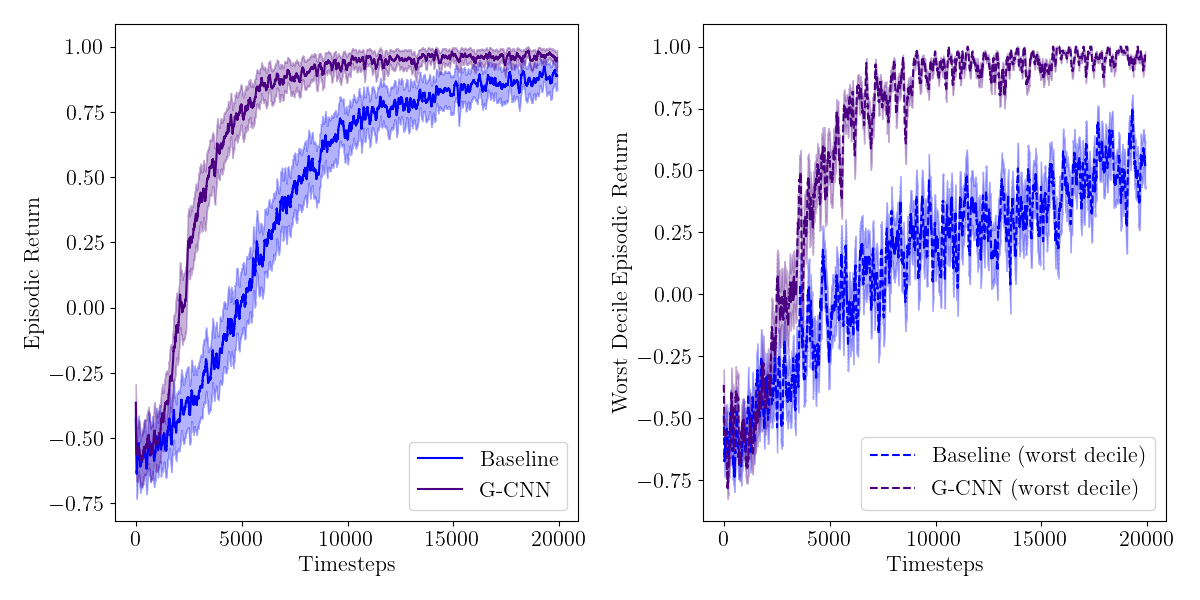
\includegraphics[width=\linewidth]{Figures/catch_returns.png}
	\caption{Left: Mean episodic returns for the Catch agents across 128 random seeds plotted against number of interaction time-steps in the MDP. Right: The mean cumulative episodic returns of the worst performing 128 random seeds against number of experience time-steps in the MDP. Both of the plots are moving averages, with windows of 10 time-steps. Additionally, two standard errors are plotted.}
\end{figure}
Upon examining the qualitative differences in the episodic return curves, we observe a familiar yet more pronounced trend. For Catch, the inductive bias of equivariance seems especially beneficial. Not only does the agent with the G-CNN converge to an expert policy more rapidly than its counterpart, but the bottom decile of random seeds also exhibits markedly improved performance. Furthermore, by referring to the tabulated results in Table~\ref{tab:actor-critic_catch}, the superiority of the Equivariant Network architecture is evident. It manages to achieve a higher proficiency in "Catch" in merely half the time compared to the alternative.
% Again, looking at the qualitative performance difference from the Episodic return curves we see a similar but more exaggerated story. For Catch the equivariance inductive bias appears to be incredibly useful, and not only does the agent converge to an expert policy faster, than without the G-CNN, but also the bottom decile of random seeds also perform substantially better. Further, looking at tabulated performance in Table~\ref{tab:actor-critic_catch}, The dominance of the Equivariant Network architecture is apparent, with it achieving a greater mastery of Catch in half of the time.

\begin{table}
	\centering
	\begin{tabular}{|c|c|c|}
		\hline
		Time-steps & Baseline         & G-CNN                     \\
		\hline
		$2, 000$   & $- 0.51\pm 0.07$ & $\mathbf{-0.06 \pm 0.09}$ \\
		$10, 000$  & $0.70 \pm 0.06$  & $\mathbf{0.95 \pm 0.03} $ \\
		$20,000$   & $0.875 \pm 0.04$ & $\mathbf{0.96\pm 0.02}$   \\
		\hline
	\end{tabular}
	\caption{Cumulative episodic returns tabulated for the two network architectures. All episodic returns are recorded with confidence intervals of two standard errors across 128 random seeds.}
	\label{tab:actor-critic_catch}
\end{table}
\subsection{Conclusion}
Equivariant actors were tested in both environments, and showed a substantially more efficient learning. These results are inline with other experiments, where agents are trained with inductive biases about the task's symmetry outperform conventional methods. Further, they also demonstrated the same improvement in cases with challenging initialization conditions.

The equivariance constraint itself however, is quite limiting. For any given task the group must be known beforehand. Not only this but it must also be an exact symmetry. In many settings these constraints are rare, especially with discrete symmetry groups.

Additionally, there is a forward pass cost to the equivariant network structure, especially with larger groups, despite the same number of parameters being used. With the way G-CNNs are constructed, the number of operations in a forward pass of the network is $\mathcal{O}(|G|)$. As such, the inference time increases when including the inductive bias. However, because these operations can be executed in parallel, the evaluation time increase is limited. For a rough estimation of the increased overhead the G-CNN. The implementations of the G-CNN for catch and the MLP were benchmarked. The MLP's mean forward pass over $10000$ states was $27.5 \pm 0.1\mu s$, and $29.9 \pm 0.1 \mu s$ for the G-CNN. This is an $8\%$ increase in evaluation time, with similar standard error across 1000 tests. An increased inference overhead is also not a problem in multiple environments such as robotic control where samples are more expensive than inference.

Despite the mild performance overhead, if a task is known to poses a discrete group symmetry, constructing a network with an inductive bias that accounts for this is demonstrably useful in increasing the training efficiency and reliability of an Agent, and should be exploited. However, the case of an exact symmetry is not universal.

The limited applicability of equivariant models motivates the next section of the report. In the case where the environment has a group structured symmetry or an approximate group structured symmetry, building an equivariant transition model may further improve the agent's learning dynamics.


